\section{実験方法}
実験手順を以下に示す. アプローチの可否は目視で判断する.
\figref{Fig:success}のようにピーマンがエンドエフェクタの収穫範囲内に入った場合は成功, \figref{Fig:failure}のように茎や葉などの収穫対象以外のものを巻き込んで把持, または切断しそうな場合は失敗とした.
\begin{enumerate}
  \item ピーマンの正面にエンドエフェクタが位置するように実験装置を配置する
  \item 実験装置をスライドさせ, ピーマン株に対して垂直方向にエンドエフェクタをアプローチさせる
  \item アプローチの可否を判断
  \begin{description}
    \item[成功条件] ピーマンがエンドエフェクタの収穫範囲内に入った場合
    \item[失敗条件] 収穫対象以外のものを巻き込んで把持, または切断しそうな場合
  \end{description}
  \item 各エンドエフェクタモデルで手順1\verb|〜|3を30個のピーマンに対して行う
  \item 実環境での成功率と設計指標から求めた成功率を比較する
\end{enumerate}

\vspace{5mm}
\begin{figure}[H]
     \centering
     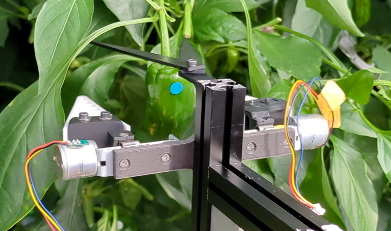
\includegraphics[width=110mm]{images/png/success.png}
     \caption{Examples of successful approaches}
     \label{Fig:success}
   \end{figure}

\begin{figure}[H]
    \centering
    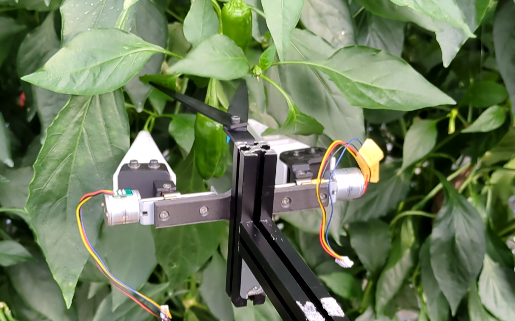
\includegraphics[width=110mm]{images/png/failure.png}
    \caption{Examples of failed approaches}
    \label{Fig:failure}
\end{figure}

設計指標から成功率を算出するため, 各エンドエフェクタモデルの成功率について考える.
各エンドエフェクタモデルがアプローチする場所は \tabref{Tab:approach}のように予想される.

\begin{table}[htbp]
  \begin{center}
    \scalebox{0.7}{
    \begin{tabular}{l|cccccc}
      Model & Front of fruit & Side of fruit & Above of fruit & Below fruit & Front of peduncle & Side of peduncle\\ \hline\hline
      Gripper type & ○ & ○ & - & - & ○ & ○\\
      Vibrating knife type & - & - & ○ & ○ & ○ & ○\\
      Peduncle approach type & - & - & - & - & ○ & ○\\
    \end{tabular}
    }
    \caption{Approach area of each model}
    \label{Tab:approach}
  \end{center}
\end{table}

これを踏まえると設計指標からの成功率は以下のようになる.

グリッパ型の成功率\\
\vspace{5mm}
$p_h = p(d_p > l_p \cap S_p > S_papproach \cap d_fside > l_fside \cap S_f > S_fapproach)$

振動ナイフ型の成功率\\
\vspace{5mm}
$p_h = p(d_p > l_p \cap S_p > S_papproach \cap d_fabove > l_fabove \cap d_funder > l_funder)$

花柄アプローチ型の成功率\\
\vspace{5mm}
$p_h = p(d_p > l_p \cap S_p > S_papproach)$

\vspace{10mm}
各エンドエフェクタモデルの計測部分を\figref{Fig:finraycad} \verb|〜| \figref{Fig:agristcad}に示す.
振動ナイフ型は下方向に刃がついているため, 正面にしかアプローチしない今回の場合はアプローチ面積をうまく表現することができない.
しかし, 刃は薄く花柄のアプローチに必要な露出面積は小さくなることが予想されるため, 結果にあまり影響がないと考え, この実験では, 花柄アプローチ面積 $h_p$ = 振動ナイフの刃の厚さとする. 

\vspace{5mm}
\begin{figure}[H]
  \centering
  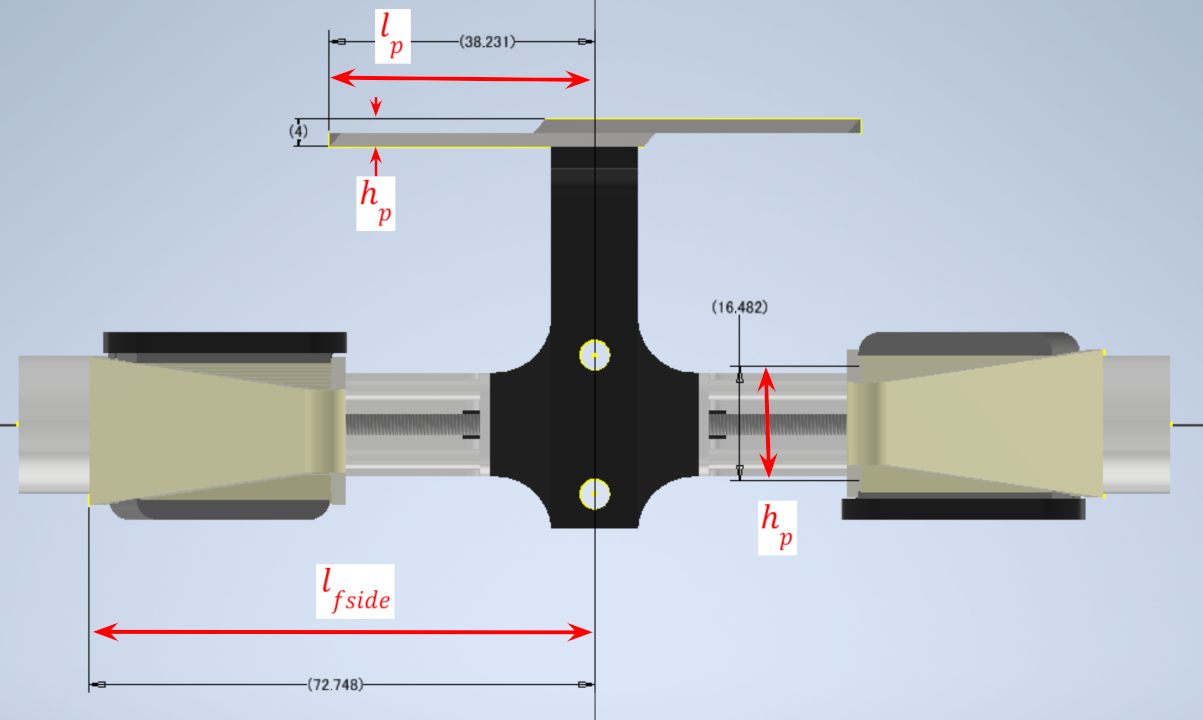
\includegraphics[width=80mm]{images/png/finraycad.png}
  \caption{Measurement of gipper type}
  \label{Fig:finraycad}
\end{figure}

\begin{figure}[H]
  \begin{minipage}[b]{0.48\columnwidth}
    \centering
    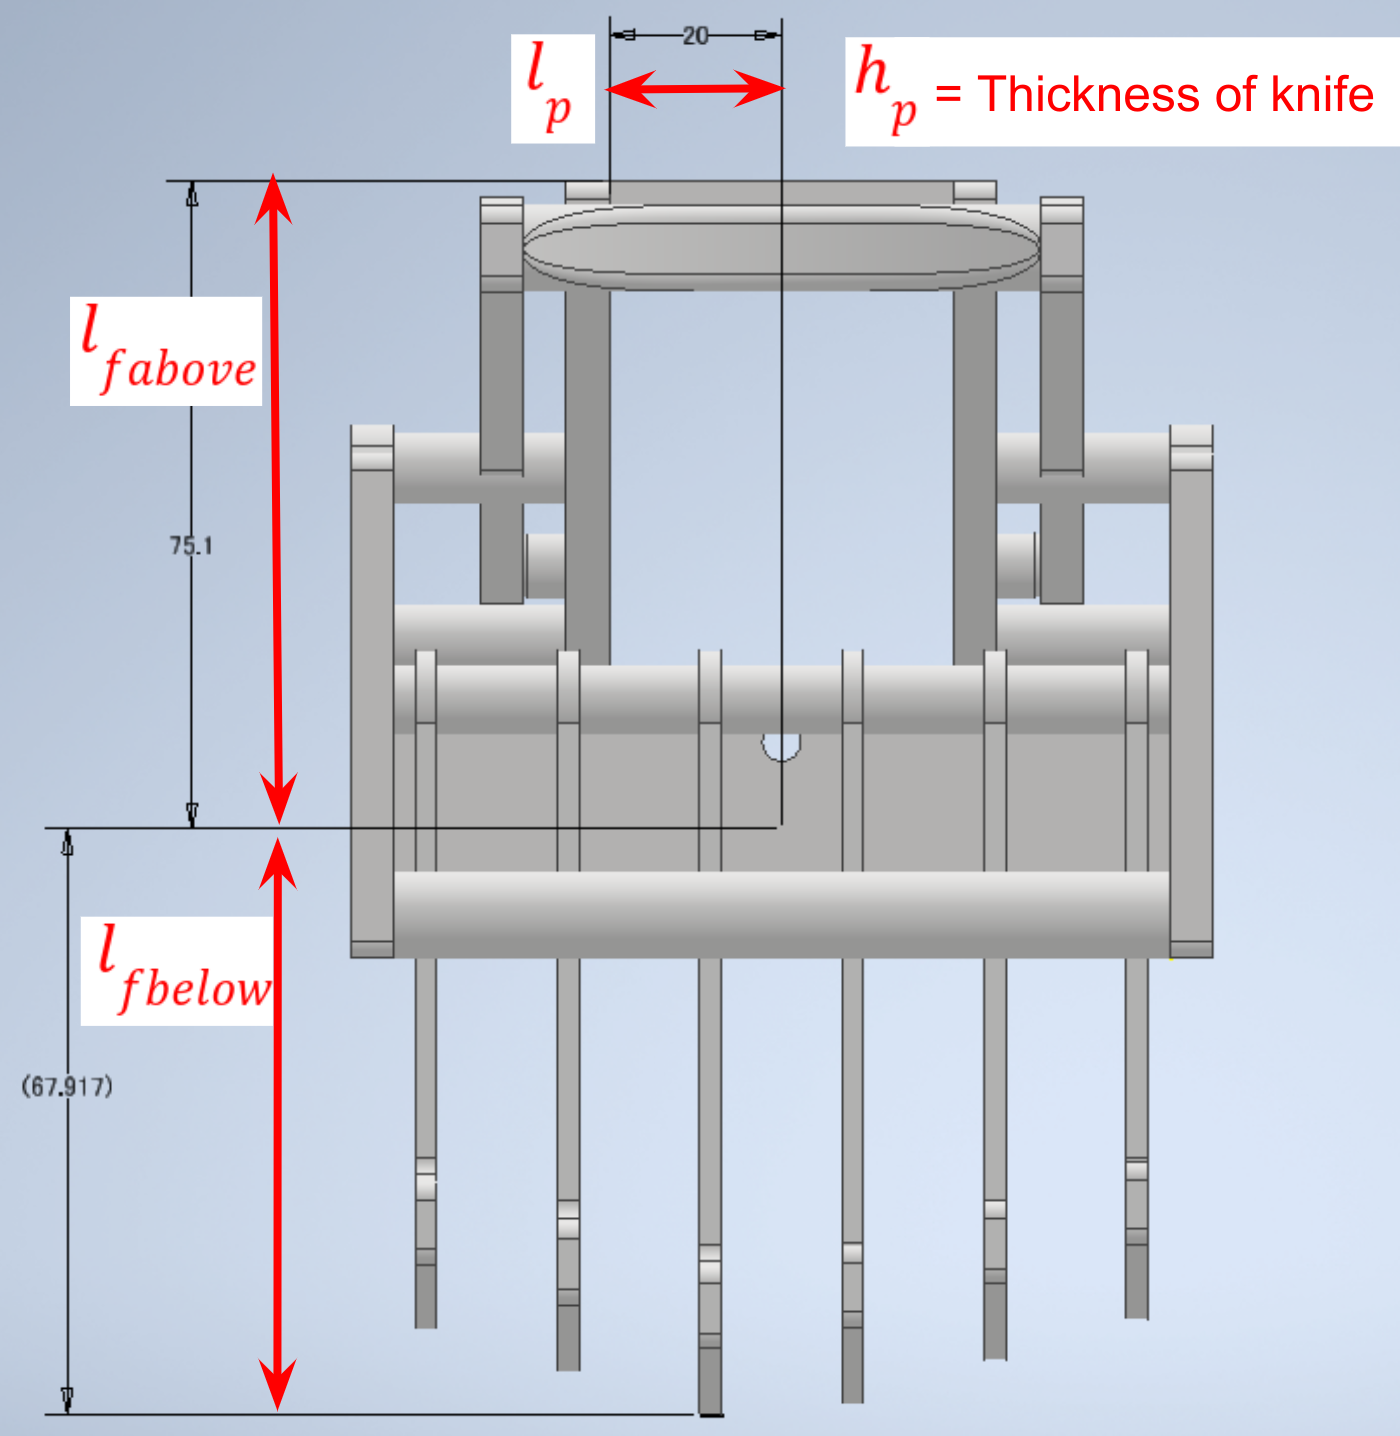
\includegraphics[width=\columnwidth]{images/png/sweepercad.png}
    \caption{Measurement of vibrating knife type}
    \label{Fig:sweepercad}
  \end{minipage}
  \hspace{0.04\columnwidth}
  \begin{minipage}[b]{0.48\columnwidth}
    \centering
    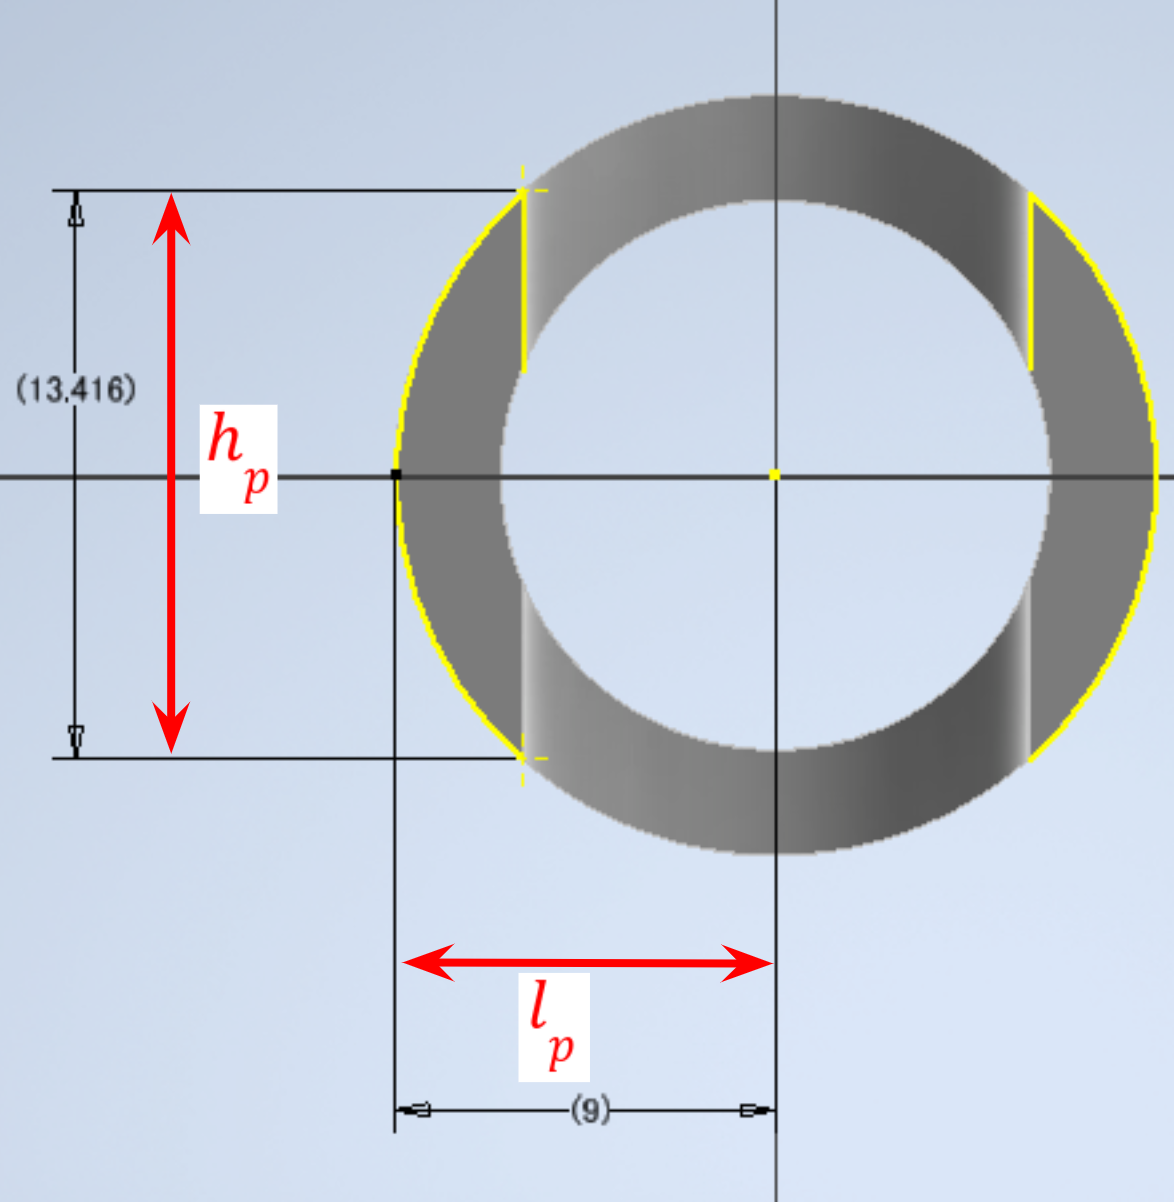
\includegraphics[width=\columnwidth]{images/png/agristcad.png}
    \caption{Measurement of peduncle approach type}
    \label{Fig:agristcad}
  \end{minipage}
\end{figure}